\documentclass{myslide}
\usepackage[slide]{mypackage}

\title{Computer System Architecture}
\subtitle{--- Computation, ISA and Datapath}

\author[chhzh123]{陈鸿峥}
\date[Dec 30, 2018]{December, 2018}

\keywords{}

\begin{document}

\begin{frame}
\titlepage
\end{frame}

\begin{frame}
\tableofcontents[hideallsubsections]
\end{frame}

\section{背景、历史、预备知识}
\begin{frame}
\sectionpage
\end{frame}

\subsection{从一切的源头讲起---计算模型}
\begin{frame}
\subsectionpage
\end{frame}

\begin{frame}{一切的开端}
\begin{center}
\large\textbf{我们必须知道,我们必将知道。}\\
\textbf{Wir m\"ussen wissen, wir werden wissen.}\\
\qquad\qquad\qquad\qquad\qquad\textbf{---大卫 希尔伯特(David Hilbert),1930}
\end{center}
\pause
希尔伯特23个问题:第二个问题 --- 算术系统的相容性
\begin{enumerate}
	\item 数学是完备的吗(complete)?% 面对那些正确的数学陈述,我们是否总能找出一个证明
	\item 数学是一致的吗(consistent)?% 数学是否没有内部矛盾
	\item 数学是可判定的吗(decidable)?% 仅仅通过机械化的计算,就能判定某个数学陈述是对是错
\end{enumerate}
\pause
\begin{itemize}[<+->]
	\item 哥德尔(G\"odel)不完备性定理, 1931
	\begin{itemize}
		\item \textbf{形式化}武器
		% 哥德尔的证明非常的长,达到了200多页纸,但其中很大的成分是用在了一些辅助性的工作上面,比如占据超过1/3纸张的是关于一个形式系统如何映射到自然数,也就是说,如何把一个形式系统中的所有公式都表示为自然数,并可以从一自然数反过来得出相应的公式。这其实就是编码,在我们现在看来是很显然的,因为一个程序就可以被编码成二进制数,反过来也可以解码。但是在当时这是一个全新的思想,也是最关键的辅助性工作之一,另一方面,这正是“程序即数据”的最初想法。
		% https://www.jianshu.com/p/9236794ddef3
		% \item 递归函数 % ($\mu$-recursive function)
		\item \textbf{一阶谓词逻辑}是完备的
	\end{itemize}
% 任何包含了算术的数学系统都不可能同时拥有完备性和一致性
% 任何包含了算术的数学系统,如果它是一致的,那么我们不能在它的内部证明它本身的一致性
% -> 在数学的领地上,有些东西我们不知道,也不可能知道。
%% 哥德尔不完备性定理告诉我们,有时候越强大的数学理论,因为能表达的概念太多,甚至连理论的命题和证明都能表达,反而会导致不能被证明的真命题的存在
	% \item 图灵(Turing)机, 1936
\end{itemize}
\end{frame}
% http://songshuhui.net/archives/70194
% http://songshuhui.net/archives/20161

\begin{frame}
\only<1->{
\begin{center}
\Large\textbf{什么是计算?}
\end{center}
}
\only<2>{
\begin{figure}
\centering
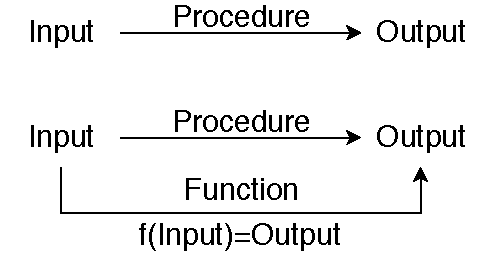
\includegraphics[width=0.6\linewidth]{fig/Lecture2/Abstraction-Computation.pdf}
\end{figure}
}
\end{frame}

% 而计算刚好解决了这个问题——计算定义了机械可以做什么,不可以做什么。如果宇宙/思想/大脑/小兔子/上帝是可以用机械的方法解释的,那么他们就是电脑,反之亦然。
\begin{frame}{图灵机}
Alan Turing, \emph{On Computable Numbers, With an Application to the Entscheidungsproblem}, 1936
\only<1>{
\begin{figure}
\centering
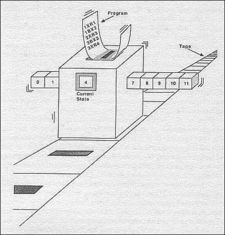
\includegraphics[width=0.25\linewidth]{fig/Lecture2/turing_machine.jpg}
\end{figure}
\begin{columns}
\begin{column}{0.5\linewidth}
\begin{itemize}
	\item 纸带(tape)
	\item 读写头(head)
	\item 状态寄存器(state register)
	\item 有限状态表(table)
\end{itemize}
\end{column}
\begin{column}{0.5\linewidth}
基本操作:
\begin{itemize}
	\item 读符号
	\item 不修改或者写符号
	\item 左移或右移纸带
\end{itemize}
\end{column}
\end{columns}
}
\only<2>{
\begin{figure}
\centering
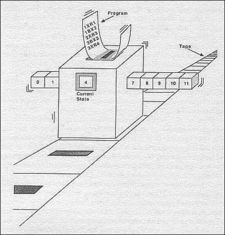
\includegraphics[width=0.25\linewidth]{fig/Lecture2/turing_machine.jpg}
\end{figure}
停机问题:是否存在这样的图灵机能够判断一个程序在给定输入上是否会停机/结束?
% “一阶谓词演算”是完备的。也就是说,在这个数学系统中,每个真理都能被证明,“真”和“能被证明”这两个概念是一致的
% 希尔伯特的可判定性问题是:是否存在一种计算过程,可以在有限步运算内,判断在这个完备的数学系统中每个命题的真假?
}
\only<3->{
\\停机问题:是否存在这样的图灵机能够判断一个程序在给定输入上是否会停机/结束?
\begin{figure}
\centering
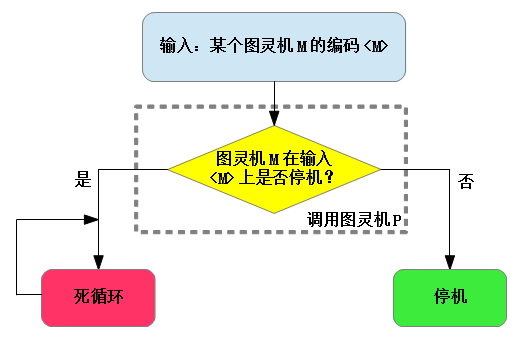
\includegraphics[width=0.5\linewidth]{fig/Lecture2/halting_problem.png}
\end{figure}
}
\only<4>{
\begin{center}
\large 即使是完备的数学系统,也是\textbf{不可判定}的!
\end{center}
}
\end{frame}
% 赋值、跳转、比较 图灵机与编程语言 - 王先生的文章 - 知乎 https://zhuanlan.zhihu.com/p/26328692

\begin{frame}{$\lambda$-Calculus}
Alonzo Church, \emph{An unsolvable problem of elementary number theory}, 1936
\only<1>{
\begin{itemize}
	\item 变量(variable):$x$
	\item 抽象(abstraction):$(\lambda x.M)$
	\item 应用(application):$(M N)$
\end{itemize}
Operation:
\begin{itemize}
	\item $\alpha$转换(conversion):$(\lambda x.M[x]) \to (\lambda y.M[y])$
	\item $\beta$规约(reduction):$((\lambda x.M) E \to (M[x\gets E]))$
\end{itemize}
}
\only<1-2>{
\begin{figure}
\centering
\begin{tabular}{cc}
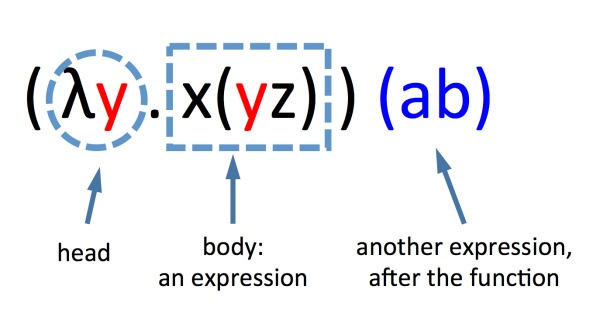
\includegraphics[width=0.5\linewidth]{fig/Lecture2/lambda_formula.jpg}&
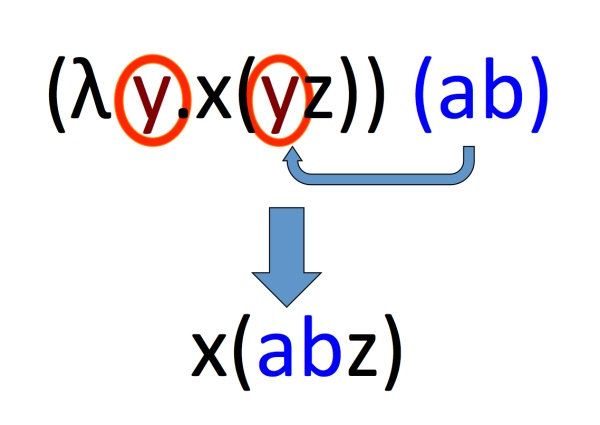
\includegraphics[width=0.4\linewidth]{fig/Lecture2/lambda_formula_2.jpg}
\end{tabular}
\end{figure}
}
\only<2>{
\begin{center}
没有\textbf{数据和程序}之分!\\
一切都是$\lambda$项,它们既是程序,也是数据
\end{center}
}
\end{frame}
% 我们甚至可以说,图灵机的设计本身,正是这些限制的一种体现。图灵很可能一开始就意识到了这些限制,再由此出发,去定义他的图灵机。哥德尔之所以对图灵机击节叹赏,大概也正因蕴含在它定义中的,图灵对“机械计算”的深刻洞察。相比之下,虽然与之等价的λ演算也尚算精致,但对于“机械计算”只得其形未得其神,显然逊色不少。
% Deutsch 所有(有限的可以实现的)物理系统都可以被一台通用计算机器来模拟。 量子计算

\begin{frame}{图灵完备}
\begin{center}
\large\textbf{图灵机与$\lambda$-演算等价!(图灵完备)}
\end{center}
\pause
\begin{center}
\fontsm
\begin{tabular}{|c|c|}\hline
命令式语言(imperative) & 函数式语言(functional)\\\hline
图灵系 & 丘奇系 \\\hline
面向计算机硬件的抽象 & 面向数学的抽象\\\hline
指令序列 & 表达式(函数是一等公民)\\\hline
C/C++/Python/Java & Lisp/Haskell/ML/Coq\\\hline
顺序执行 & 对求值顺序不相关,易于并行\\
有副作用,依赖外部环境(如IO) & 无副作用,纯函数,不出现竞争冒险\\
变量对应着存储单元 & 变量只是代数名称\\\hline
\end{tabular}
\end{center}
\pause
若不考虑内存的限制,绝大多数编程语言都是图灵完备的
\end{frame}

\begin{frame}{计算模型}
\begin{center}
\Large\textbf{什么是可计算的?(Computability)}
\end{center}
\pause
\begin{center}
\Large\textbf{Church-Turing Thesis}\\
\large所有可以有效计算的函数都可以被通用图灵机计算
\end{center}
\begin{itemize}
	\item \textbf{机械计算}就是图灵机能做的计算 $\gets$ 可计算理论的基石 % 希尔伯特在他的问题中那模糊的“机械计算”
	\item \textbf{目前}任何计算装置(乃至大脑、超算)都不能超过图灵机的能力(不考虑速度,只考虑可计算性)
\end{itemize}
\end{frame}
% 一阶逻辑 形式验证
% 密码学
% 函数式编程
% 计算复杂性理论

\begin{frame}
\begin{center}
\Large\textbf{怎么去计算?}
\end{center}
\end{frame}

\begin{frame}
\begin{center}
$\lambda$-演算 更像是智慧的推理\\
\quad\\
而 图灵机 真正抓住了 {\Large\textbf{机械计算}} 的神韵
\end{center}
\end{frame}

\subsection{冯诺依曼体系结构}
\begin{frame}
\subsectionpage
\end{frame}

% \begin{frame}
% ENIAC, 第一台电子计算机
% 十进制计算,逻辑元件多,结构复杂,可靠性低
% 不是存储程序式的计算机,编程通过手工插接线方式进行
% \end{frame}

\begin{frame}{冯诺依曼体系结构}
\begin{itemize}
	\item 图灵机是\textbf{理论}的最简单的模型,但具有非常强的计算力
	\item 冯诺依曼(von Neumann)体系结构则是对图灵机的物理\textbf{实现}(EDVAC, 1945)
\end{itemize}
% EDVAC, 1945, 第一台现代意义的通用计算机, 首次用二进制
\begin{figure}
\centering
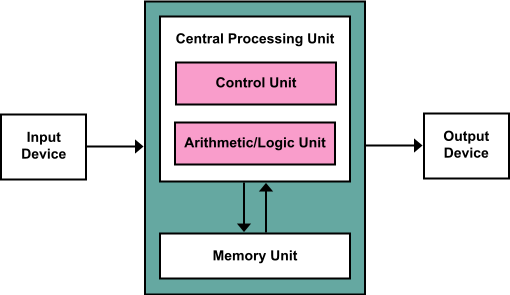
\includegraphics[width=0.5\linewidth]{fig/Lecture2/Von_Neumann_Architecture.png}
\end{figure}
\begin{itemize}[<+->]
	\item \textbf{存储器!}二进制!
	\item 所有指令与数据都\textbf{无区别}地存储在计算机中
\end{itemize}
\end{frame}

\subsection{数据的表示与大小}
\begin{frame}
\subsectionpage
\end{frame}

\begin{frame}[fragile]{数据的表示}
数据的表示
\begin{itemize}
	\item 原码(sign-magnitude):最高位为符号位
	\item 反码(\textbf{ones'} complement):负数按位取反
	\item 补码(\textbf{two's} complement):模$2^n$运算,反码+1
\end{itemize}
进制
\begin{itemize}
	\item 二进制\verb'0b10'
	\item 八进制\verb'034'
	\item 十六进制\verb'0xFF'或\verb'FFH'
\end{itemize}
\end{frame}

\begin{frame}{基本数据单位}
数据单位
\begin{itemize}
	\item 位(bit):处理信息的最小单位
	\item 字节(Byte):存储的基本单位,$1$B$=8$bit
	\item 字(Word):随机器而变,32位机 $1$Word$=4$B$=32$bit
	\item 字长(Word length):数据通路的宽度/字的长度
\end{itemize}
内存大小\\
\begin{center}
1KiB=$2^{10}$B\qquad
1MiB=$2^{10}$KiB\qquad
1GiB=$2^{10}$MiB
\end{center}
\end{frame}

\section{指令集系统概述}
\begin{frame}
\sectionpage
\end{frame}

\subsection{指令集背景}
\begin{frame}[fragile]{指令集背景}
\only<1>{
\begin{center}
\begin{tikzcd}
\text{Machine Language (Binary)[1945]}
\end{tikzcd}
\end{center}
}
\only<2>{
\begin{center}
\begin{tikzcd}
\text{Assembly Language [1947]}\arrow{d}{Assembler[1948]}\\
\text{Machine Language (Binary)[1945]}
\end{tikzcd}
\end{center}
}
\only<3>{
\begin{center}
\begin{tikzcd}
\text{Natural language}\arrow{d}\\
\text{High-Level Programming Language (FORTRAN)[1954]}\arrow{d}{\text{Compiler}[1954]}\\
\text{Assembly Language [1947]}\arrow{d}{\text{Assembler}[1948]}\\
\text{Machine Language (Binary)[1945]}
\end{tikzcd}
\end{center}
}
\only<4>{
\begin{center}
\begin{tikzcd}
\text{Natural language}\arrow{d}\\
\text{High-Level Programming Language (FORTRAN)[1954]}\arrow{d}{\text{Compiler}[1954]}\\
\text{Assembly Language [1947]}\arrow{d}{\text{Assembler}[1948]}\\
\text{Machine Language (Binary)[1945]}
\end{tikzcd}
\end{center}
}
\only<5>{
\begin{columns}
\begin{column}{0.65\linewidth}
\begin{center}
\begin{tikzcd}
\text{Natural language}\arrow{d}\\
\text{High-Level Programming Language [1954]}\arrow{d}{\text{Compiler}[1954]}\\
\text{Assembly Language [1947]}\arrow{d}{\begin{tabular}{l}\fontsm\text{Assembler[1948]}\\\fontsm\text{\textcolor{red}{Instruction Set Architecture (ISA)[1970s]}}\end{tabular}}\\
\text{Machine Language (Binary)[1945]}
\end{tikzcd}
\end{center}
\end{column}
\begin{column}{0.35\linewidth}
Assembly:\\
add \$1, \$0, 1 \\
sw \$1, \$0(4) \\
\quad\\
Machine:\\
0000 0010 1100 0111 \\
0001 1101 0100 1000
\end{column}
\end{columns}
}
\end{frame}

\subsection{指令系统的作用}
\begin{frame}{指令系统概述}
\begin{figure}
\centering
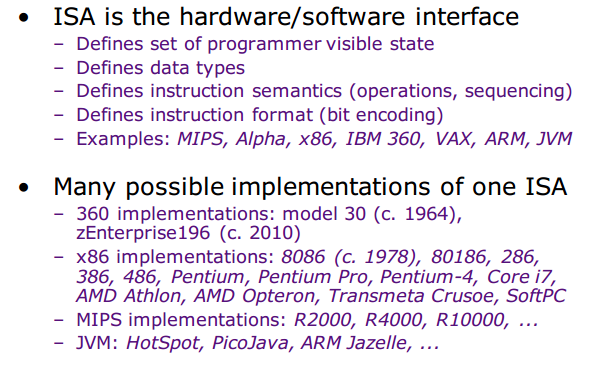
\includegraphics[width=0.9\linewidth]{fig/Lecture2/overview.PNG}
\end{figure}
\end{frame}

\begin{frame}{指令系统的作用}
\begin{itemize}
	\item 硬件设计者角度:
	\begin{itemize}
		\item ISA为CPU提供功能需求
		\item ISA设计目标:易于硬件逻辑设计
	\end{itemize}
	\item 系统程序员角度:
	\begin{itemize}
		\item 通过ISA使用硬件资源
		\item ISA设计目标:易于编写编译器
	\end{itemize}
\end{itemize}
\begin{center}
\textbf{ISA determines the performance and the cost of computers}
\end{center}
\end{frame}

\subsection{指令集计算机}
\begin{frame}[fragile]{指令集计算机}
\begin{center}
\begin{tabular}{|p{5cm}|p{5cm}|}
\hline
\multicolumn{1}{|c|}{\textbf{复杂指令集计算机}} & \multicolumn{1}{c|}{\textbf{精简指令集计算机}} \\\hline
CISC, Complex Instruction Set Computer & RISC, Reduce Instruction Set Computer\\\hline
出现较早(1970s),大而全 & 出现较晚(1980s),小而精 \\\hline
指令周期长,专用寄存器,微程序控制,难编译优化生成高效目标代码,效率低 & 指令周期短,大量通用寄存器,组合逻辑电路控制,优化编译系统\\\hline
变长指令字 & 定长指令字 \\\hline
x86 & ARM(Advanced RISC Machine), MIPS, SPARC \\\hline
\end{tabular}
\end{center}
\end{frame}

\begin{frame}{处理器性能评价}
\begin{figure}
\centering
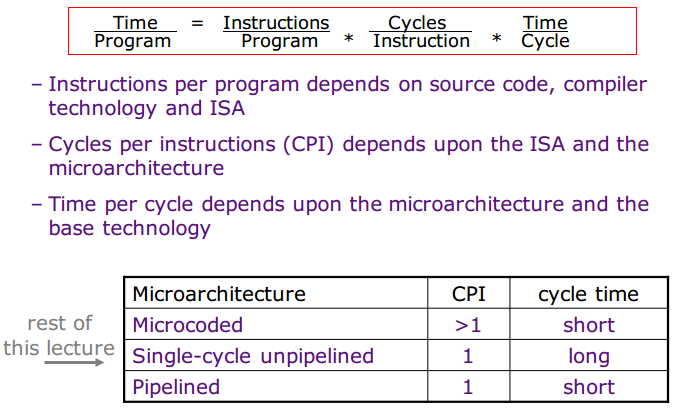
\includegraphics[width=\linewidth]{fig/Lecture2/processor_performance.PNG}
\end{figure}
\# of instructions, cycles, CPI
\end{frame}

\subsection{指令集系统基本内容}
\begin{frame}{指令集系统}
\begin{enumerate}
	\item 什么操作?操作码
	\item 操作对象?操作数
	\item 如何找到操作对象?寻址方式 % 4字节=32位
\end{enumerate}
指令=操作码+地址码
\end{frame}

\begin{frame}{指令集系统}
\begin{enumerate}
	\item 数据传送指令:store、load
	\item 算术运算指令:加减乘除
	\item 逻辑运算指令:与或非
	\item 输出输出指令:I/O
	\item 系统控制指令:启动IO设备、存取特殊寄存器指令
	\item 程序控制指令:转移、跳转、返回、中断
\end{enumerate}
\end{frame}


\section{RISC-V指令集总览}
\begin{frame}
\sectionpage
\end{frame}

\begin{frame}{RISC-V指令集}
\begin{itemize}
	\item 所有指令都是32位宽(4字节),按字地址对齐
	\item 基本的RV32I共47条指令
\end{itemize}
\end{frame}
% P35
% 32 位字节可寻址的地址空间
% 所有指令均为 32 位长
% 31 个寄存器,全部 32 位宽,寄存器 0 硬连线为零
% 所有操作都在寄存器之间(没有寄存器到内存的操作)
% 加载/存储字加上有符号和无符号加载/存储字节和半字
% 所有算术,逻辑和移位指令都有立即数版本的指令
% 立即数总是符号扩展
% 仅提供一种数据寻址模式(寄存器+立即数)和 PC 相对分支
% 无乘法或除法指令(RV32M扩展)
% 一个指令,用于将大立即数加载到寄存器的高位,这样加载 32 位常量到寄存器只需要两条指令
% 大量可用的指令码空间

\begin{frame}[fragile]{Registers}
\verb'x1-x31', \verb'x0'=0, Program Counter (PC)
\begin{columns}
\begin{column}{0.3\linewidth}
\begin{figure}
\centering
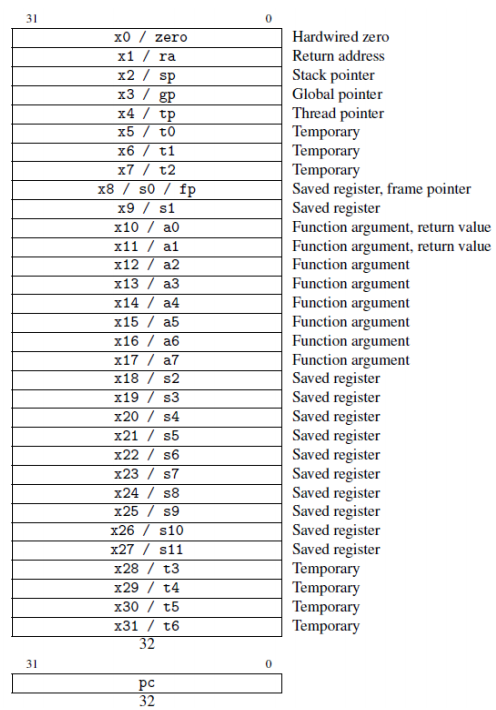
\includegraphics[width=\linewidth]{fig/Lecture2/general_registers.PNG}
\end{figure}
\end{column}
\begin{column}{0.6\linewidth}
\begin{itemize}
	\item RISC-V共32个通用寄存器,有零寄存器,且PC不是通用寄存器
	\item x86-32仅8个寄存器,且无零寄存器
	\item arm-32有16个寄存器,但PC不作为单独寄存器
\end{itemize}
\end{column}
\end{columns}
\end{frame}
% 伪指令 jump return beqz

\begin{frame}{Instruction Formats}
\only<1>{
\begin{figure}
\centering
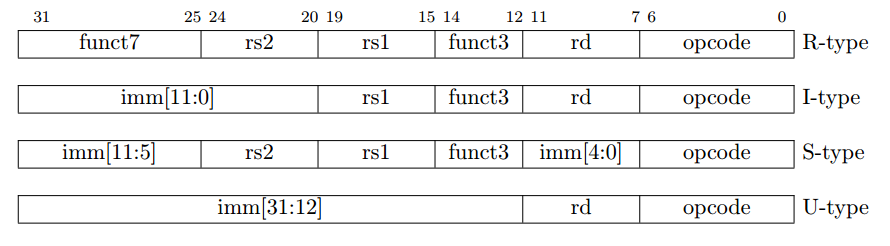
\includegraphics[width=\linewidth]{fig/Lecture2/rvi_formats.PNG}
\end{figure}
}
\only<2>{
\begin{figure}
\centering
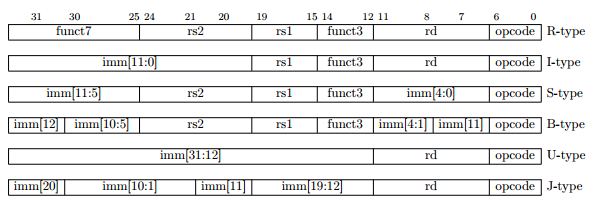
\includegraphics[width=\linewidth]{fig/Lecture2/rvi_formats_complex.PNG}
\end{figure}
}
\begin{itemize}
	\item rs1, rs2, rd are at the same position (MIPS is not)
	\item Immediates are put leftmost, sign 31 (sign-extension can be done before ID)
	\item 12bits regular + 20bits load upper
	\item Only has sign-extended imm
	\item The last bit used for extension (64-bit)
\end{itemize}
\end{frame}

\section{单周期CPU}
\begin{frame}
\sectionpage
\end{frame}

\subsection{Introduction}
\begin{frame}
\subsectionpage
\end{frame}

\begin{frame}{Central Processor Unit (CPU)}
\begin{figure}
\centering
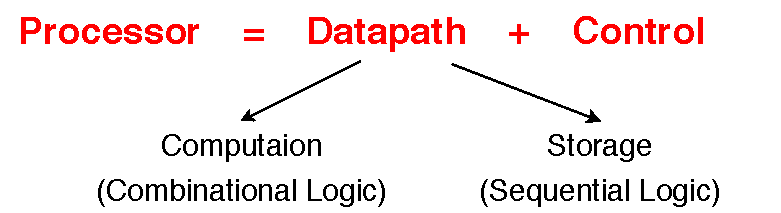
\includegraphics[width=0.8\linewidth]{fig/Lecture2/Abstraction-Processor.pdf}
\end{figure}
\end{frame}

\begin{frame}{CPU指令执行过程}
2-phases:
\begin{enumerate}
	\item Fetch phase
	\item Execute phase
\end{enumerate}
5-stages CPU:
\begin{enumerate}
	\item Instruction Fetch (IF)
	\item Instruction Decode (ID)
	\item Execution (EXE)
	\item Access memory (MEM)
	\item Write back (WB)
\end{enumerate}
\end{frame}

\begin{frame}[fragile]{核心指令}
\begin{columns}
\begin{column}{0.5\linewidth}
Main instructions:
\begin{enumerate}
	\item \verb'add rd, rs1, rs2'
	\item \verb'addi rd, rs, imm'
	\item \verb'lw rd, rs(imm)'
	\item \verb'sw rs, rd(imm)'
	\item \verb'beq rd, rs, offset'
	\item \verb'j address'
\end{enumerate}
\end{column}
\begin{column}{0.5\linewidth}
Examples:
\begin{itemize}
	\item \verb'add $3, $2, $1'
	\item \verb'add $3, $2, 10'
	\item \verb'lw $3, $2(4)'
	\item \verb'sw $3, $2(4)'
	\item \verb'beq $3, $2, -2'
	\item \verb'j 0x00000050'
\end{itemize}
\end{column}
\end{columns}
\end{frame}

\subsection{Some Basic Modules}
\begin{frame}
\subsectionpage
\end{frame}

\begin{frame}
\begin{center}
All problems in computer science can be solved by another\\
\quad\\
{\textbf{\huge{abstraction}}} layer.\\
\quad\\
隐藏low-level细节,给high-level提供简单模型
\end{center}
\end{frame}

\begin{frame}{布尔逻辑层}
0-1: 布尔运算能够用物理器件模拟(如继电器、二极管等等)
\pause
\begin{center}
物理电路层$\to$布尔逻辑层
\end{center}
\end{frame}

\begin{frame}{计算器件层}
1-2: 基本数学运算能够用布尔运算模拟
\only<1-2>{
\begin{columns}
\begin{column}{0.4\linewidth}
\begin{center}
\begin{tabular}{|c|c|c|c|}\hline
A & B & A+B & Carry\\\hline
0 & 0 & 0 & 0\\\hline
0 & 1 & 1 & 0\\\hline
1 & 0 & 1 & 0\\\hline
1 & 1 & 0 & 1\\\hline
\end{tabular}
\end{center}
\pause
\[\begin{aligned}
A+B &= A\oplus B\\
Carry &= AB
\end{aligned}\]
\end{column}
\begin{column}{0.6\linewidth}
\begin{figure}
\centering
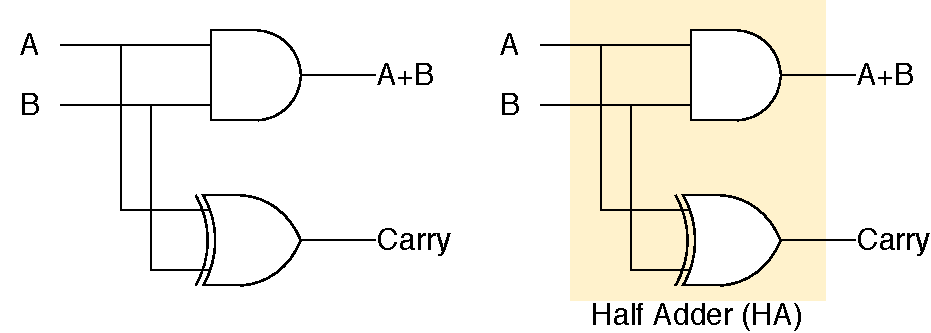
\includegraphics[width=\linewidth]{fig/Lecture2/Abstraction-HA.pdf}
\end{figure}
\end{column}
\end{columns}
}
\only<3>{
\begin{figure}
\centering
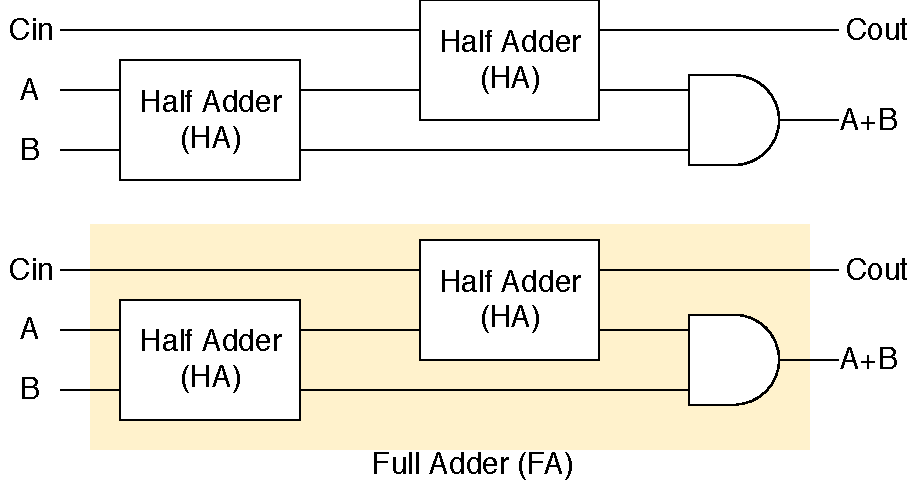
\includegraphics[width=0.8\linewidth]{fig/Lecture2/Abstraction-FA.pdf}
\end{figure}
}
\only<4-5>{
\begin{figure}
\centering
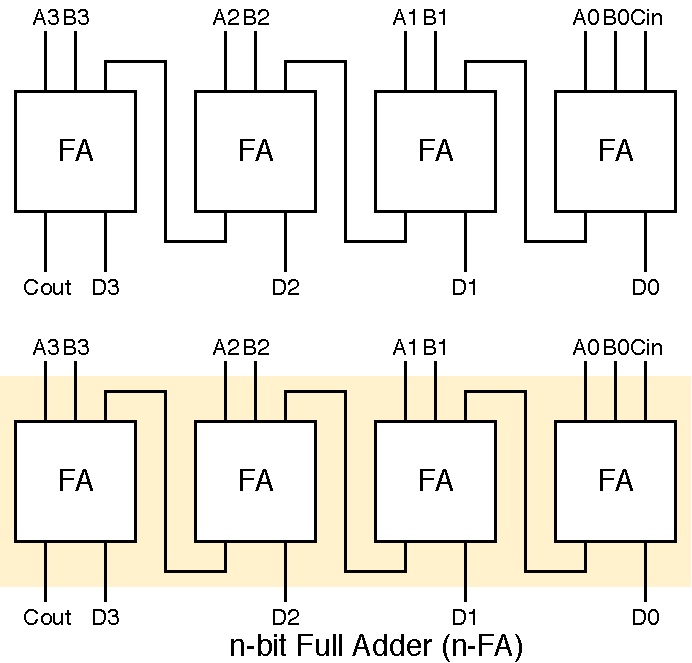
\includegraphics[width=0.4\linewidth]{fig/Lecture2/Abstraction-nFA.pdf}
\end{figure}
}
\pause
\begin{center}
物理电路层$\to$布尔逻辑层$\to$计算器件\textbf{(组合逻辑)}
\end{center}
\end{frame}

\begin{frame}{计算器件层(时序逻辑)}
\begin{columns}
\begin{column}{0.5\linewidth}
\begin{figure}
\centering
\begin{tabular}{c}
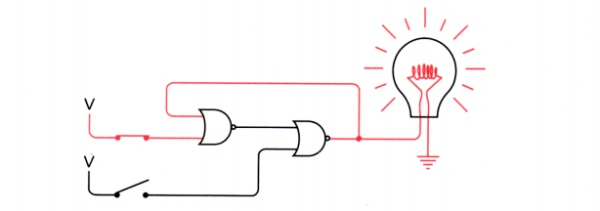
\includegraphics[width=\linewidth]{fig/Lecture2/ff_1.jpg}\\
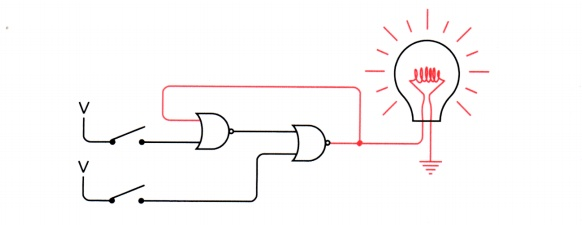
\includegraphics[width=\linewidth]{fig/Lecture2/ff_2.jpg}
\end{tabular}
\end{figure}
\end{column}
\pause
\begin{column}{0.5\linewidth}
\begin{figure}
\centering
\begin{tabular}{c}
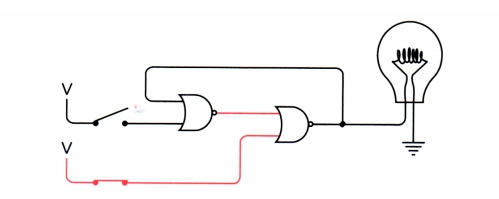
\includegraphics[width=\linewidth]{fig/Lecture2/ff_3.jpg}\\
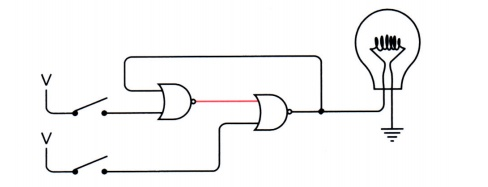
\includegraphics[width=\linewidth]{fig/Lecture2/ff_4.jpg}
\end{tabular}
\end{figure}
\end{column}
\end{columns}
\pause
\begin{center}
\Large\textbf{锁存器(Latch)!记忆信息!}
\end{center}
\end{frame}

\begin{frame}{计算器件层(时序逻辑)}
\begin{figure}
\centering
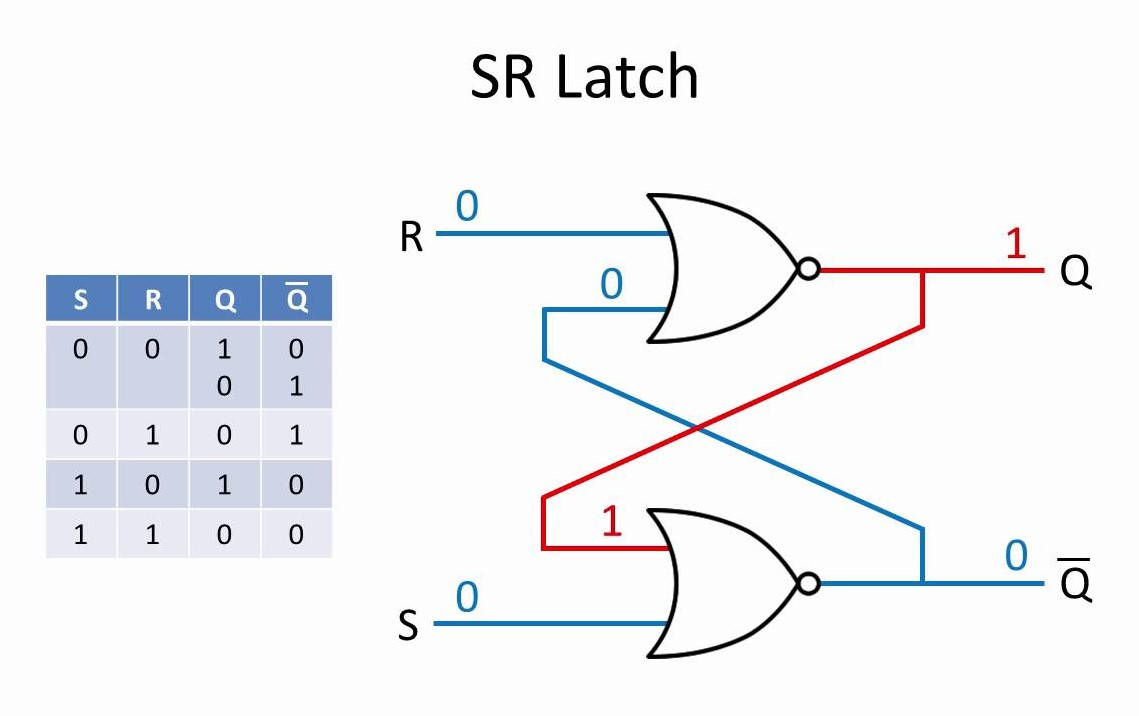
\includegraphics[width=0.8\linewidth]{fig/Lecture2/sr-latch.jpg}
\end{figure}
\end{frame}

\begin{frame}{计算器件层(时序逻辑)}
\begin{center}
\large D Latch
\end{center}
\begin{figure}
\centering
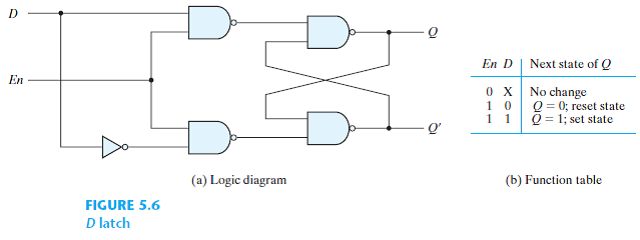
\includegraphics[width=0.9\linewidth]{fig/Lecture2/d-latch.png}
\end{figure}
\end{frame}

\begin{frame}{计算器件层(时序逻辑)}
\begin{center}
\large D Flip-flop (触发器) -- 对\textbf{时钟边沿}敏感
\end{center}
\begin{figure}
\centering
\begin{tabular}{cc}
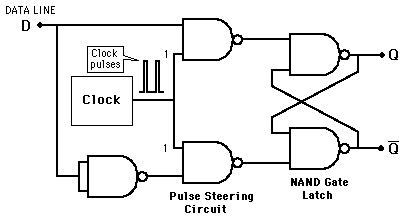
\includegraphics[width=0.6\linewidth]{fig/Lecture2/d-ff.png}&
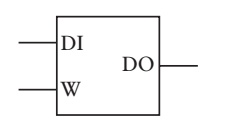
\includegraphics[width=0.3\linewidth]{fig/Lecture2/d-ff_2.jpg}
\end{tabular}
\end{figure}
\end{frame}

\begin{frame}{计算器件层(时序逻辑)}
\begin{figure}
\centering
\begin{tabular}{c}
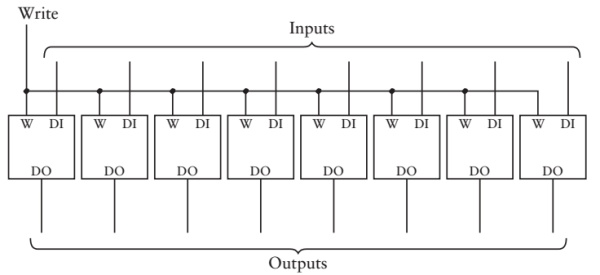
\includegraphics[width=0.8\linewidth]{fig/Lecture2/8bit-latch.jpg}\\
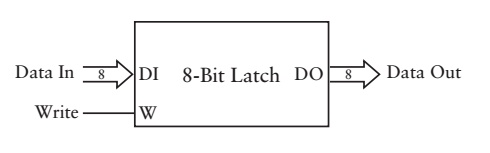
\includegraphics[width=0.6\linewidth]{fig/Lecture2/8bit-latch_2.jpg}
\end{tabular}
\end{figure}
\end{frame}

\begin{frame}{计算器件层}
8-1 Multiplexer
\begin{figure}
\centering
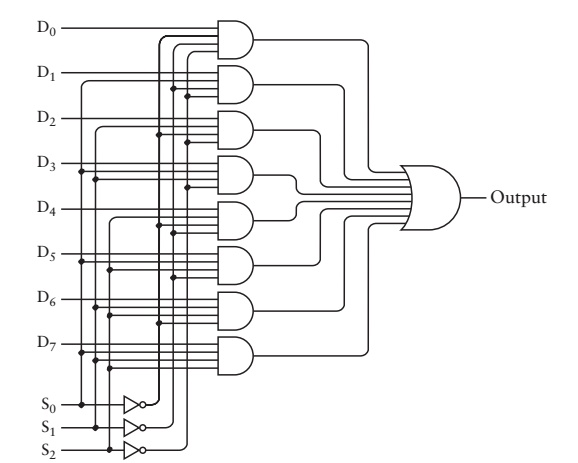
\includegraphics[width=0.6\linewidth]{fig/Lecture2/8-1mux.jpg}
\end{figure}
\end{frame}

\begin{frame}{计算器件层}
3-8 Decoder
\begin{figure}
\centering
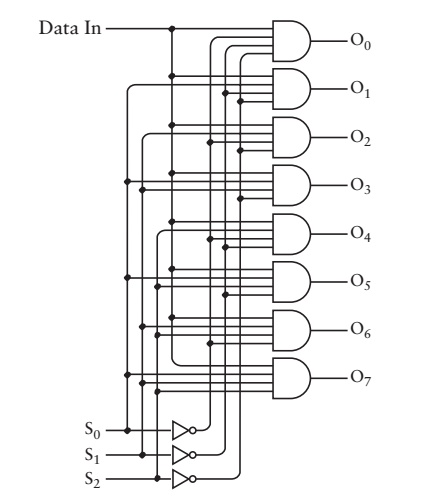
\includegraphics[width=0.5\linewidth]{fig/Lecture2/3-8decoder.jpg}
\end{figure}
\end{frame}

\begin{frame}{计算器件层}
8-bit Memory (RAM)
\begin{figure}
\centering
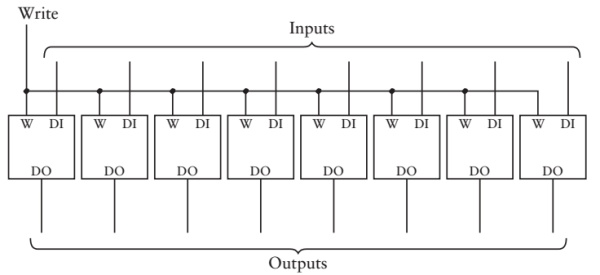
\includegraphics[width=0.8\linewidth]{fig/Lecture2/8bit-latch.jpg}
\end{figure}
\end{frame}

\begin{frame}{计算器件层}
寄存器堆 (Register File)
\begin{figure}
\centering
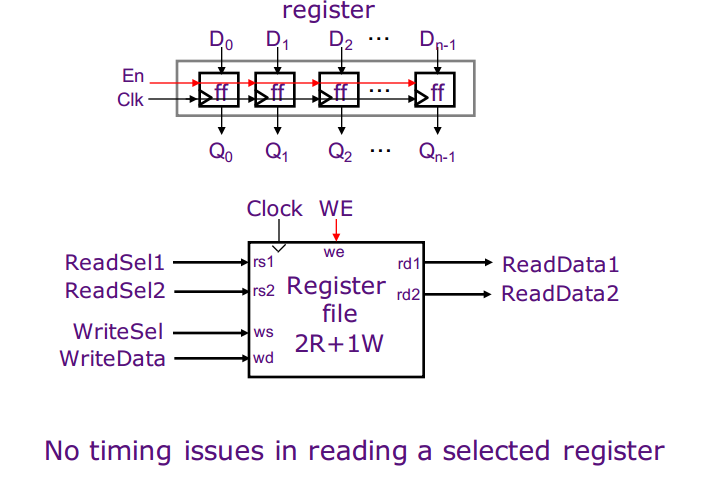
\includegraphics[width=0.8\linewidth]{fig/Lecture2/register_files.PNG}
\end{figure}
\end{frame}

\begin{frame}
0-2: 从理论到实践的第一步
\begin{center}
物理电路层$\to$布尔逻辑层$\to$计算器件/模块
\end{center}
\pause
2-3: 用基本器件实现通用处理器(CPU)
\begin{center}
\Large\textbf{架构层}
\end{center}
\end{frame}

\subsection{Common Datapath}
\begin{frame}
\subsectionpage
\end{frame}

\begin{frame}[fragile]{共同通路(PC)}
Program Counter (PC)
\begin{columns}
\begin{column}{0.5\linewidth}
\begin{figure}
\centering
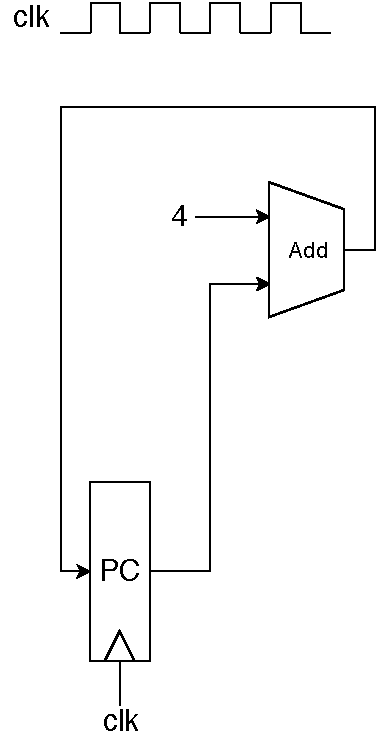
\includegraphics[width=0.5\linewidth]{fig/Lecture2/Datapath-PC.pdf}
\end{figure}
\end{column}
\begin{column}{0.5\linewidth}
按字编址\\
\verb'0x00000000'\\
\verb'0x00000004'\\
\verb'0x00000008'\\
\verb'0x0000000C'\\
$\cdots$
\end{column}
\end{columns}
\end{frame}

\subsection{R-R Instructions}
\begin{frame}
\subsectionpage
\end{frame}

\begin{frame}[fragile]{Register-Register Instructions}
\begin{figure}
\centering
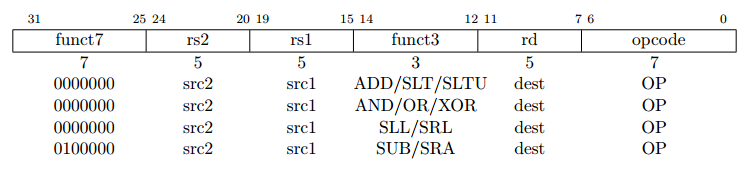
\includegraphics[width=\linewidth]{fig/Lecture2/r-r.PNG}
\end{figure}
\begin{itemize}
	\item \verb'add rd, rs1, rs2'
	\item \verb'and rd, rs1, rs2'
	\item \verb'sll rd, rs1, rs2'
	\item \verb'sub rd, rs1, rs2'
\end{itemize}
\end{frame}
% xor x1,x1,x2
% xor x2,x1,x2
% xor x1,x1,x2

\begin{frame}{Register-Register Instructions}
\begin{figure}
\centering
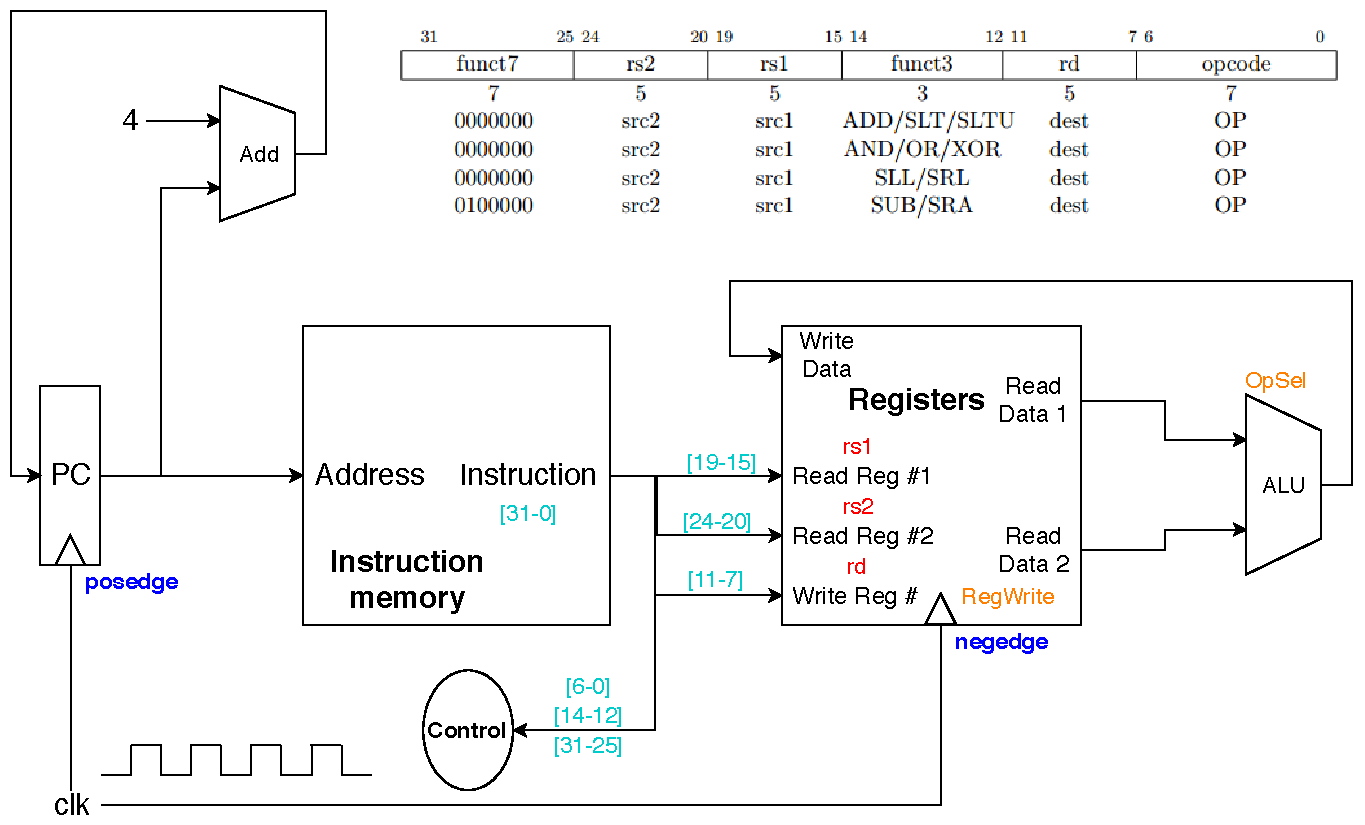
\includegraphics[width=\linewidth]{fig/Lecture2/Datapath-R-R.pdf}
\end{figure}
\end{frame}

\begin{frame}{Arithmetic Logic Unit (ALU)}
\begin{center}
\begin{tabular}{|c|l|}
    \hline
    OpSel[2:0] & \multicolumn{1}{c|}{Function}\\
    \hline
    000   & $Y=A+B$\\
    \hline
    001   & $Y=A-B$\\
    \hline
    010   & $Y=B<<A$ \\
    \hline
    011   & $Y=A\mid B$\\
    \hline
    100   & $Y=A\& B$\\
    \hline
    101   & $Y=(A<B)\;?\;1\;:\;0$\\
    \hline
    110   & \multicolumn{1}{p{7cm}|}{$\begin{aligned}
    Y&=(((A<B) \&\& (A[31] == B[31] ))\\
    &||\quad( ( A[31] ==1 \&\& B[31] == 0)))\\
    &?\;1\;:\;0
    \end{aligned}$}\\
    \hline
    111   & $Y=A\oplus B$\\
    \hline
\end{tabular}
\end{center}
\end{frame}

\begin{frame}[fragile]{Register-Register Instructions}
NO OPERATION (NOP)\\
\verb'nop' $\to$ \verb'addi x0, x0, 0'\\
doesn't change any user-visible state, except for advancing PC
\begin{figure}
\centering
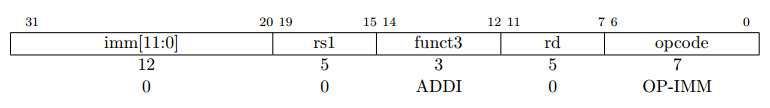
\includegraphics[width=\linewidth]{fig/Lecture2/nop.PNG}
\end{figure}
\end{frame}

\subsection{R-I Instructions}
\begin{frame}
\subsectionpage
\end{frame}

\begin{frame}[fragile]{Register-Immediate Instructions}
\begin{figure}
\centering
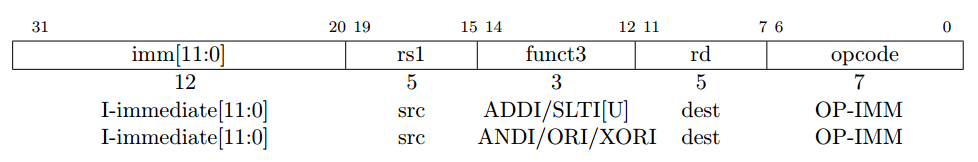
\includegraphics[width=\linewidth]{fig/Lecture2/r-i.PNG}
\end{figure}
All \textbf{sign-extended}
\begin{itemize}
	\item \verb'addi rd, rs1, imm' $\to$ imm=0, \verb'mv rd, rs1'
	\item \verb'sltiu rd, rs1, imm' $\to$ imm=1, \verb'seqz rd, rs'
	\item \verb'xori rd, rs1, imm' $\to$ imm=-1, \verb'not rd, rs'
\end{itemize}
\end{frame}

\begin{frame}[fragile]{Register-Immediate Instructions}
\begin{figure}
\centering
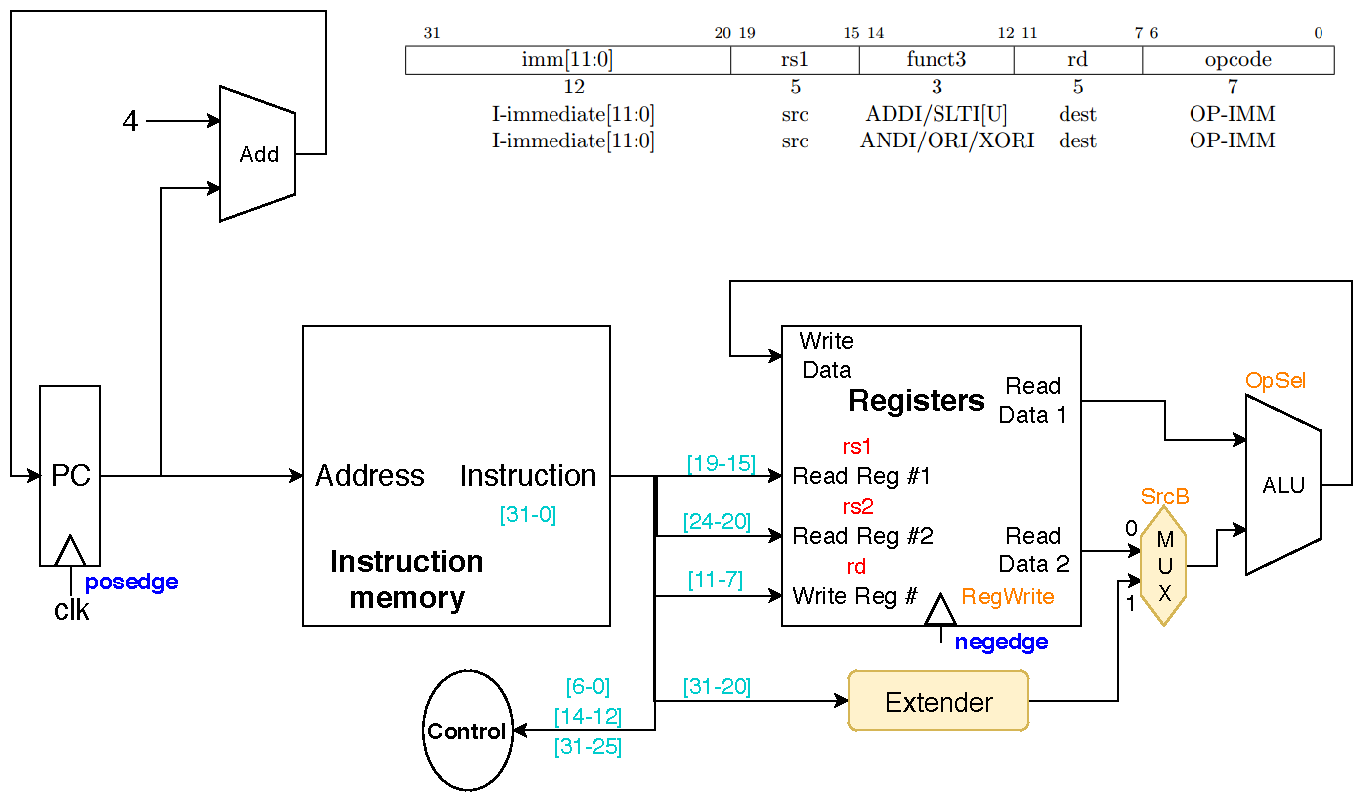
\includegraphics[width=\linewidth]{fig/Lecture2/Datapath-R-I.pdf}
\end{figure}
\end{frame}

\begin{frame}[fragile]{Register-Immediate Instructions}
\begin{figure}
\centering
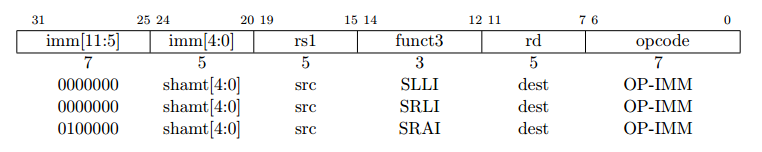
\includegraphics[width=\linewidth]{fig/Lecture2/r-i_2.PNG}
\end{figure}
\begin{itemize}
	\item Shift left (logic): \verb'slli rd, rs1, imm'
	\item Shift right (logic): \verb'srli rd, rs1, imm'
	\item Shift right (arithmetic): \verb'srai rd, rs1, imm'
	\item Need not \verb'slai'
\end{itemize}
\end{frame}
% slli rd, rs1, shamt x[rd] = x[rs1] ≪ shamt
% 立即数逻辑左移(Shift Left Logical Immediate). I-type, RV32I and RV64I.
% 把寄存器x[rs1]左移shamt位,空出的位置填入0,结果写入x[rd]。对于RV32I,仅当shamt[5]=0时,指令才是有效的。
% srai rd, rs1, shamt x[rd] = (x[rs1] ≫𝑠 shamt)
% 立即数算术右移(Shift Right Arithmetic Immediate). I-type, RV32I and RV64I.
% 把寄存器 x[rs1]右移 shamt 位,空位用 x[rs1]的最高位填充,结果写入 x[rd]。对于 RV32I,仅当 shamt[5]=0 时指令有效。

\begin{frame}[fragile]{Register-Immediate Instructions}
\begin{figure}
\centering
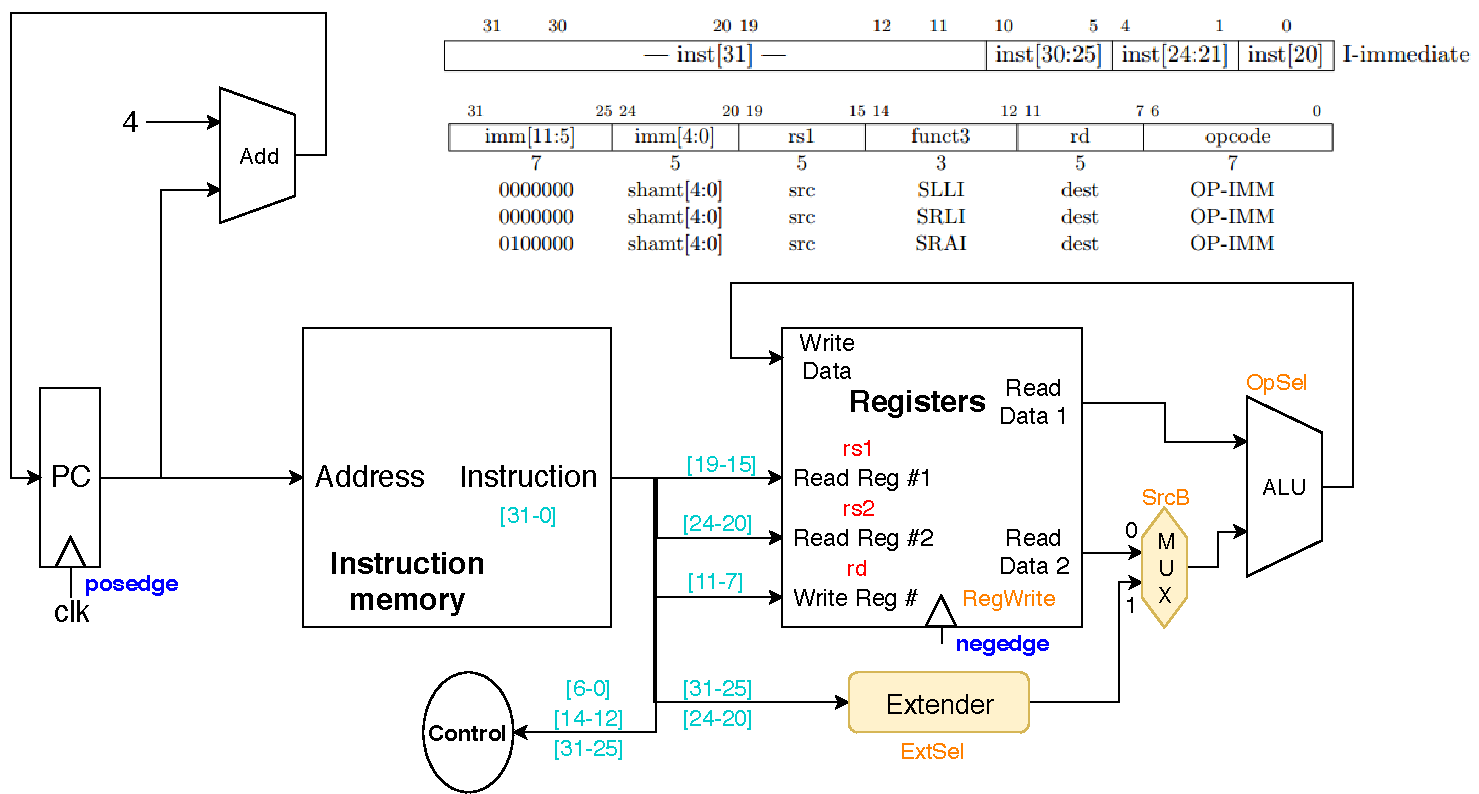
\includegraphics[width=\linewidth]{fig/Lecture2/Datapath-R-I_2.pdf}
\end{figure}
Problem unfixed: How to extend for \verb'srai'? Or set a threshold in ALU?
\end{frame}

\begin{frame}[fragile]{Immediates format}
\begin{figure}
\centering
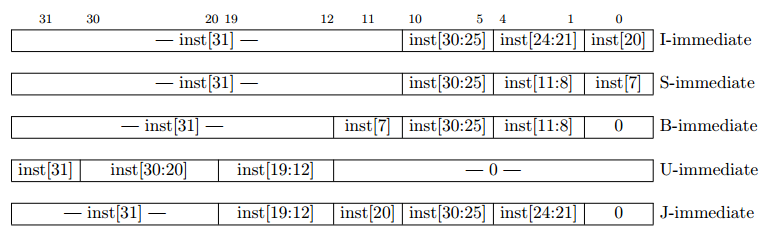
\includegraphics[width=\linewidth]{fig/Lecture2/imm.PNG}
\end{figure}
shift uses I-immediate
\end{frame}

\subsection{Load and Store}
\begin{frame}
\subsectionpage
\end{frame}

\begin{frame}[fragile]{两种存储方式}
\begin{itemize}
	\item 小端(Little-endian)存储: \textbf{RISC-V}、x86、iOS、Android
	\item 大端(Big-endian)存储: MIPS、JPEG、Photoshop
\end{itemize}
\begin{center}
\verb'0x12345678'\qquad
\begin{tabular}{ccccc}
Address & 00 & 04 & 08 & 0C\\\hline
Little & 78 & 56 & 34 & 12\\\hline
Big & 12 & 34 & 56 & 78\\\hline
\end{tabular}
\end{center}
无边界对齐(misaligned)!提供细粒度访问(半字节)
\begin{figure}
\centering
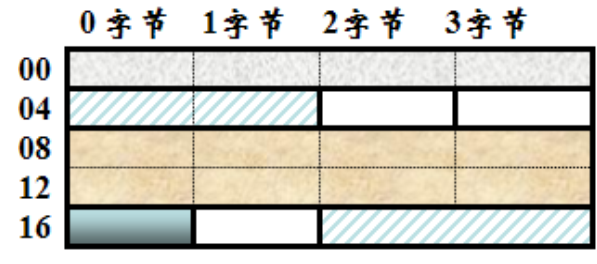
\includegraphics[width=0.4\linewidth]{fig/Lecture2/aligned.PNG}
\end{figure}
\end{frame}

\begin{frame}[fragile]{Load \& Store}
RISC-V is \textbf{Load-Store Architecture}, only \verb'lw' and \verb'sw' can access memory\\
Other arithmetic instructions can only operate on CPU registers
\begin{figure}
\centering
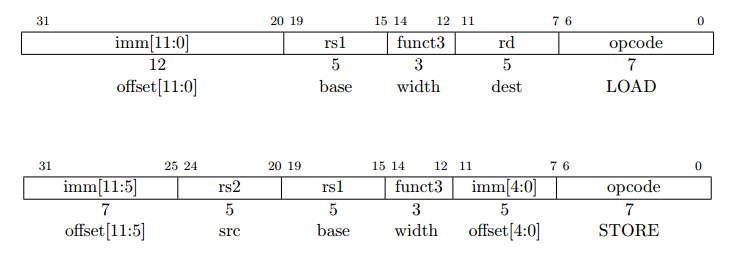
\includegraphics[width=\linewidth]{fig/Lecture2/lw-sw.PNG}
\end{figure}
\begin{itemize}
	\item \verb'lw rd, base(imm)'
	\item \verb'sw rs, base(imm)'
\end{itemize}
\end{frame}

\begin{frame}[fragile]{Load}
\verb'x[rd] = sgnext(M[x[rs1] + sgnext(offset)][31:0])'
\begin{figure}
\centering
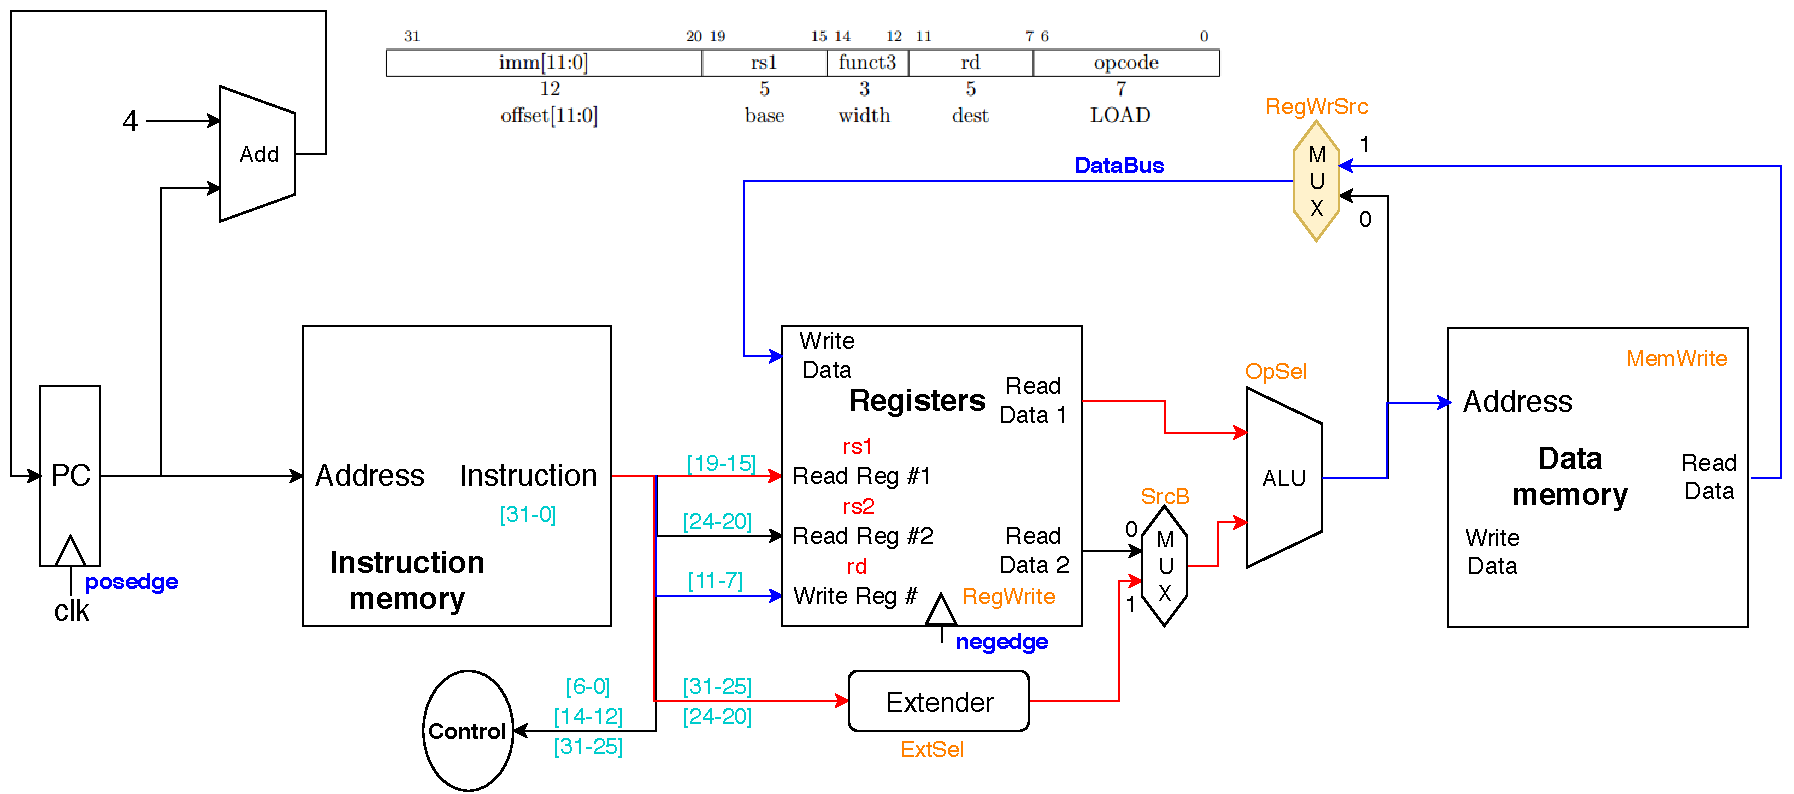
\includegraphics[width=\linewidth]{fig/Lecture2/Datapath-lw.pdf}
\end{figure}
\end{frame}
% 字加载 (Load Word). I-type, RV32I and RV64I.
% 从地址 x[rs1] + sign-extend(offset)读取四个字节,写入 x[rd]。对于 RV64I,结果要进行符号位扩展。

\begin{frame}[fragile]{Store}
\verb'M[x[rs1] + sgnext(offset)] = x[rs2][31:0]'
\begin{figure}
\centering
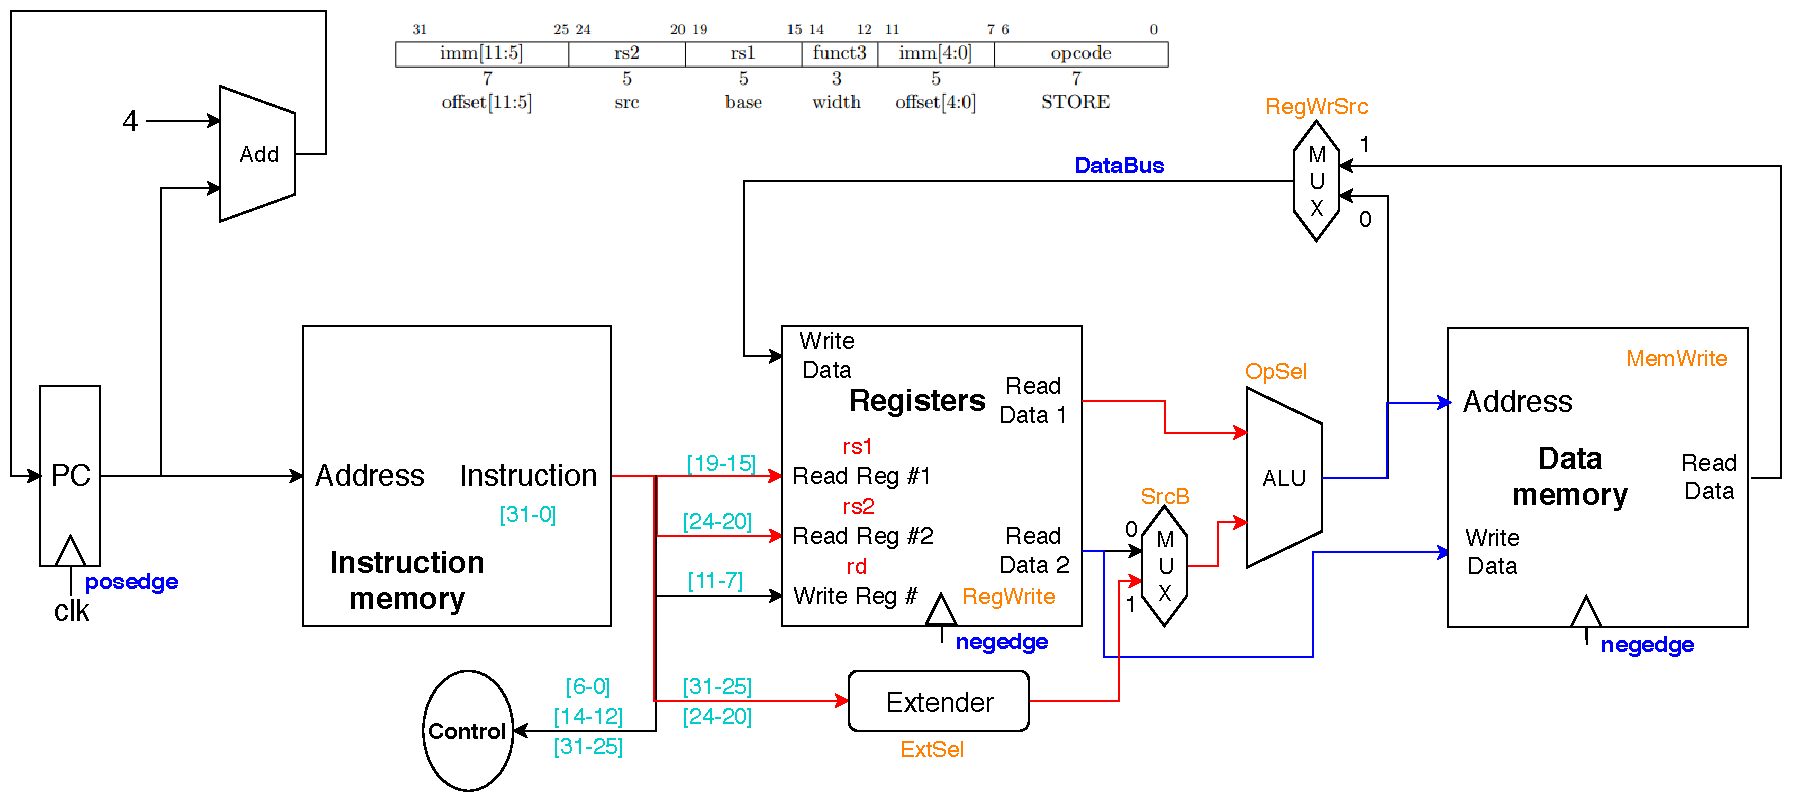
\includegraphics[width=\linewidth]{fig/Lecture2/Datapath-sw.pdf}
\end{figure}
\end{frame}
% 存字(Store Word). S-type, RV32I and RV64I.
% 将 x[rs2]的低位 4 个字节存入内存地址 x[rs1]+sign-extend(offset)。

\subsection{Branch}
\begin{frame}
\subsectionpage
\end{frame}

\begin{frame}[fragile]{Branch}
\begin{itemize}
	\item Used in loop
	\item Important for pipelining (Branch prediction)
	\item address range $\pm 4$KiB
\end{itemize}
\begin{figure}
\centering
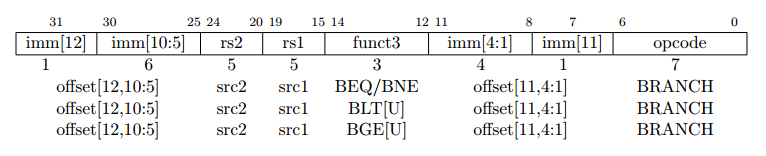
\includegraphics[width=\linewidth]{fig/Lecture2/branch.PNG}
\end{figure}
\begin{itemize}
	\item \verb'beq rs1, rs2, imm'
\end{itemize}
\end{frame}

\begin{frame}[fragile]{Branch}
\fontsm \verb'if (rs1 == rs2) pc += sgnext(offset)'偏移量均为2的倍数,但地址必须4的倍数,否则抛异常
\begin{figure}
\centering
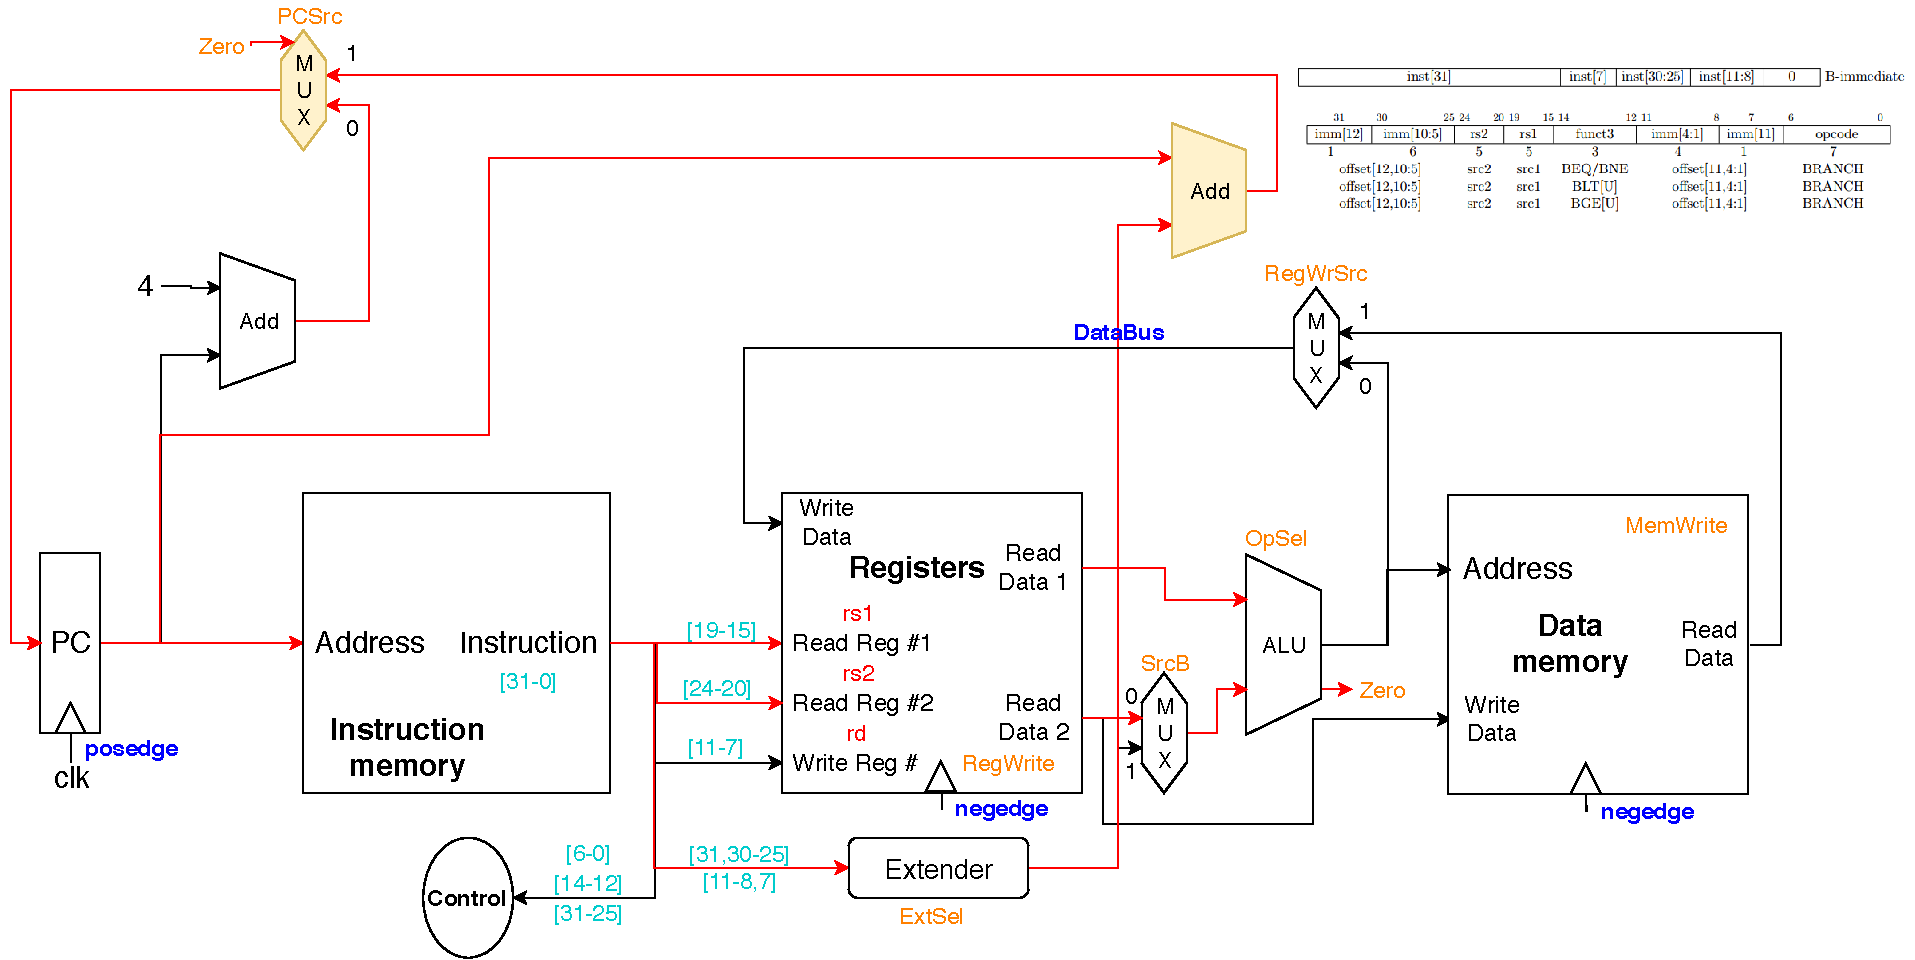
\includegraphics[width=\linewidth]{fig/Lecture2/Datapath-branch.pdf}
\end{figure}
Use ExtSel (maybe 3 bits) to control which type of imm
\end{frame}
% 相等时分支 (Branch if Equal). B-type, RV32I and RV64I.
% 若寄存器 x[rs1]和寄存器 x[rs2]的值相等,把 pc 的值设为当前值加上符号位扩展的偏移 offset。

\subsection{Jump}
\begin{frame}
\subsectionpage
\end{frame}

\begin{frame}{Function Call}
堆栈、保护现场、恢复现场
\begin{figure}
\centering
\begin{tabular}{cc}
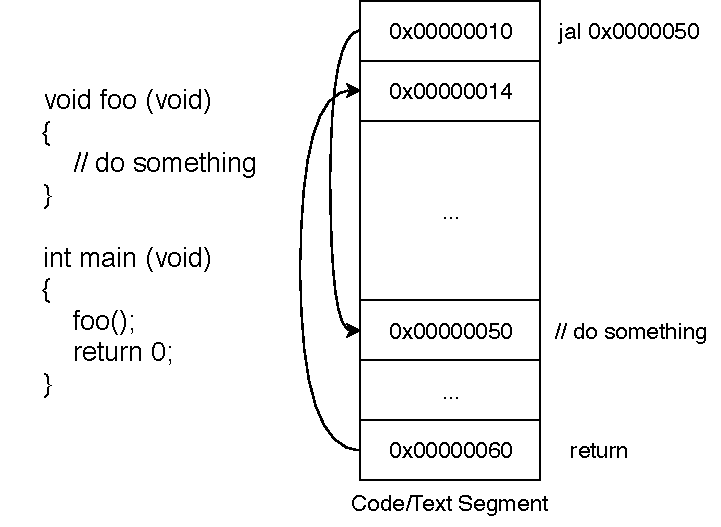
\includegraphics[width=0.5\linewidth]{fig/Lecture2/Abstraction-Function_Call.pdf}&
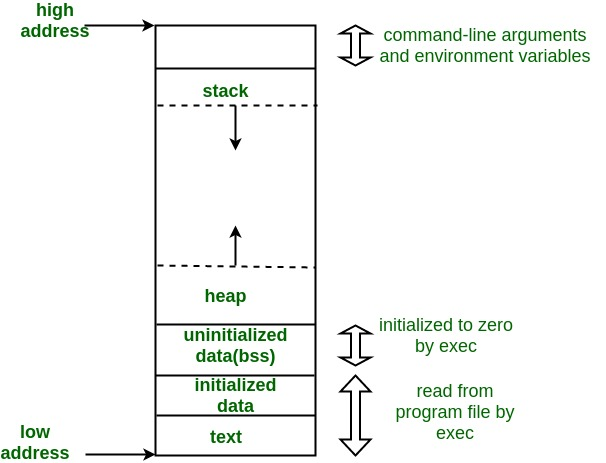
\includegraphics[width=0.5\linewidth]{fig/Lecture2/memoryLayoutC.jpg}
\end{tabular}
\end{figure}
\end{frame}

\begin{frame}[fragile]{Jump}
Address range $\pm 1$MiB
\begin{figure}
\centering
\begin{tabular}{c}
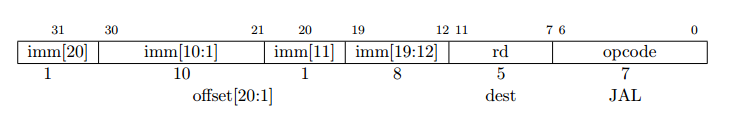
\includegraphics[width=\linewidth]{fig/Lecture2/jal.PNG}\\
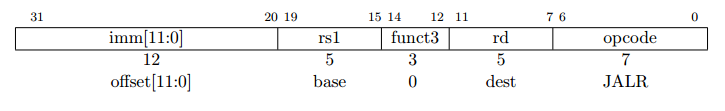
\includegraphics[width=\linewidth]{fig/Lecture2/jalr.PNG}
\end{tabular}
\end{figure}
\begin{itemize}
	\item \verb'jal rd, offset'
	\item \verb'jalr rd, offset(rs1)'
\end{itemize}
Use \verb'lui' and \verb'auipc' to jump anywhere in a 32-bit pc-relative address range
\end{frame}

\begin{frame}[fragile]{Jal}
\fontsm\verb'x[rd] = pc+4; pc += sgnext(offset)'
\begin{figure}
\centering
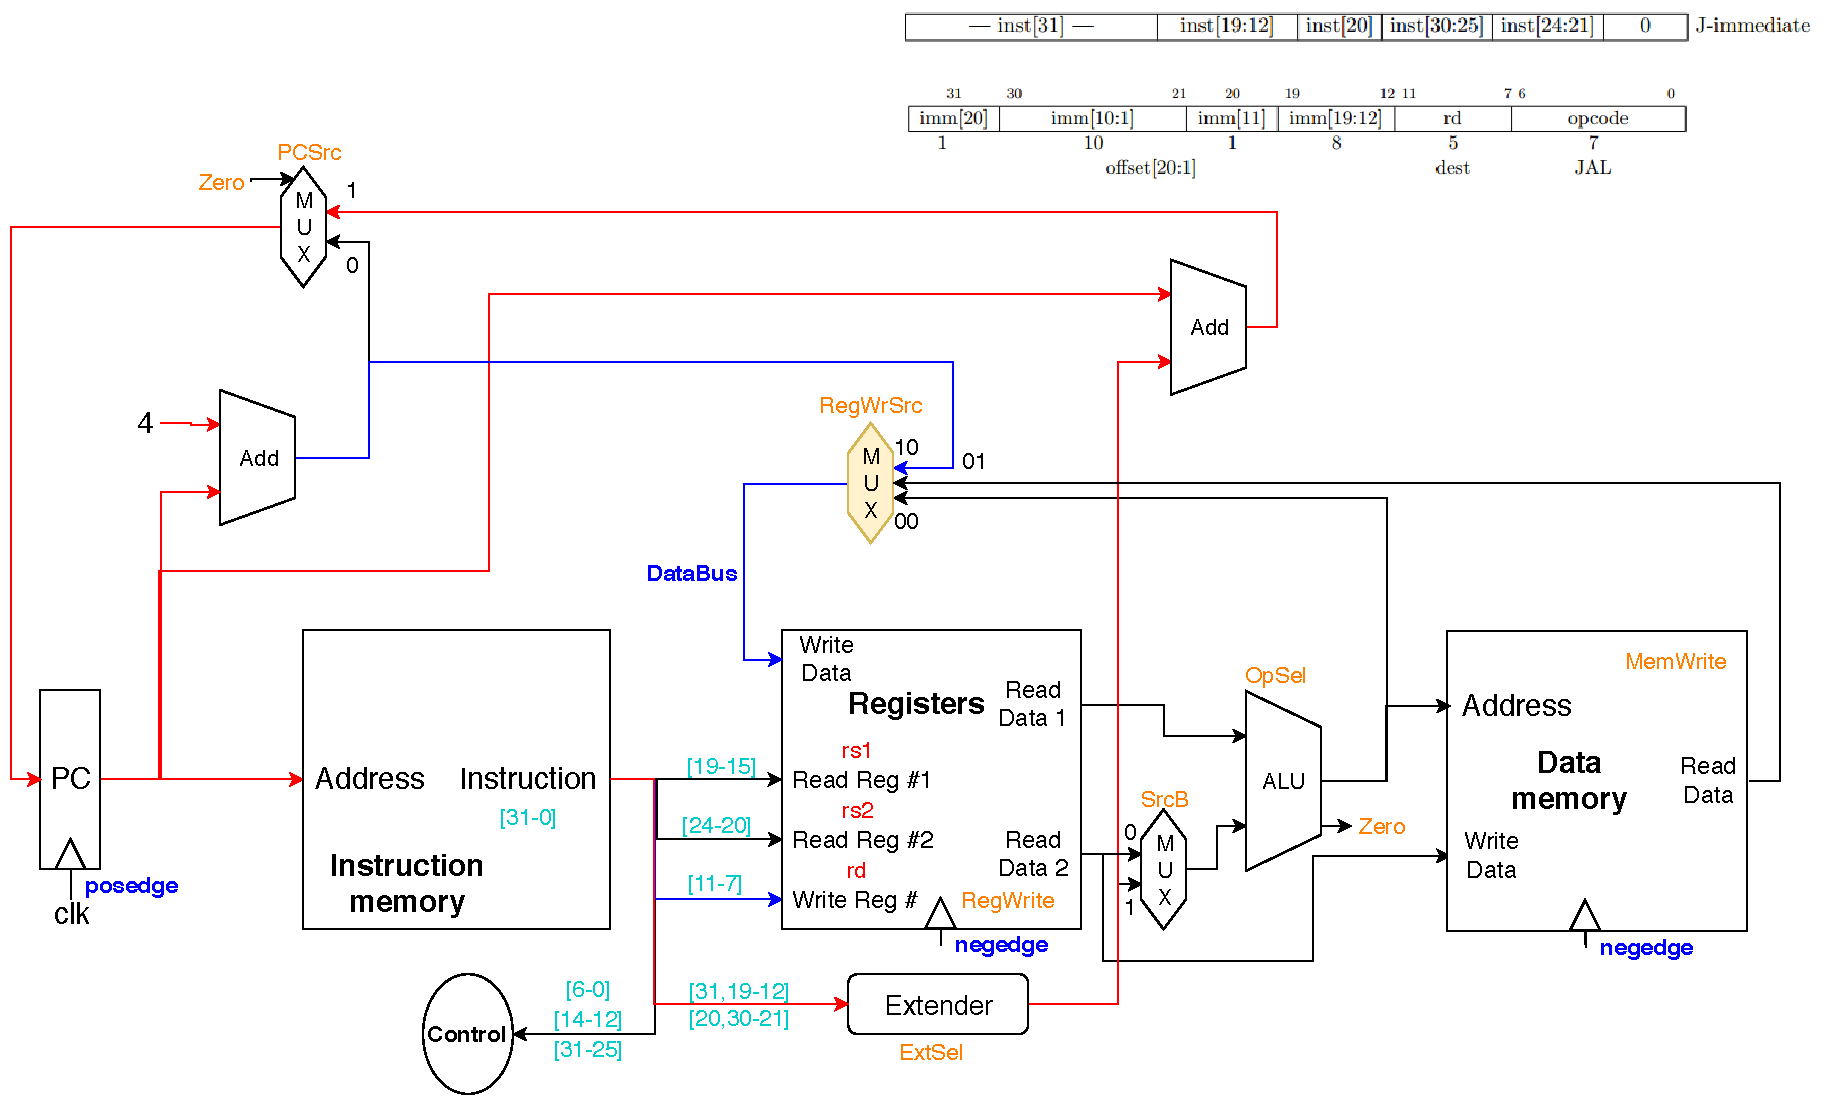
\includegraphics[width=0.8\linewidth]{fig/Lecture2/Datapath-jal.pdf}
\end{figure}
\end{frame}
% 跳转并链接 (Jump and Link). J-type, RV32I and RV64I.
% 把下一条指令的地址(pc+4),然后把 pc 设置为当前值加上符号位扩展的 offset。rd 默认为 x1。

\begin{frame}[fragile]{Jalr}
% \verb't=pc+4; pc=(x[rs1]+sext(offset))&~1; x[rd]=t'
\fontsm{\verb'x[rd]=pc+4; pc=(x[rs1]+sext(offset))&~1;' 偏移量同样是2的倍数,地址非4的倍数抛异常}
\begin{figure}
\centering
\includegraphics[width=0.8\linewidth]{fig/Lecture2/Datapath-jalr.pdf}
\end{figure}
Question again: Where to implement \verb'&~1'?
\end{frame}
% 跳转并寄存器链接 (Jump and Link Register). I-type, RV32I and RV64I.
% 把 pc 设置为 x[rs1] + sign-extend(offset),把计算出的地址的最低有效位设为 0,并将原 pc+4的值写入 f[rd]。 rd 默认为 x1。

\subsection{Single Cycle CPU Summary}
\begin{frame}
\subsectionpage
\end{frame}

\begin{frame}{Harvard Architecture (Aiken and Mark)}
Separate program and data memory
\begin{figure}
\centering
\includegraphics[width=\linewidth]{fig/Lecture2/Datapath-All.pdf}
\end{figure}
\end{frame}

\begin{frame}{Control Signals}
Hardwired control is pure combinational logic
\begin{figure}
\centering
\includegraphics[width=0.5\linewidth]{fig/Lecture2/Datapath-Control-signals.pdf}
\end{figure}
\end{frame}

\begin{frame}{Princeton Architecture (von Neumann)}
The same program and data memory
\begin{figure}
\centering
\includegraphics[width=\linewidth]{fig/Lecture2/Datapath-Princeton.pdf}
\end{figure}
\end{frame}

\begin{frame}{State Transition}
Two-state controller (A filp-flop can be used to remember)
\begin{figure}
\centering
\includegraphics[width=0.4\linewidth]{fig/Lecture2/Datapath-State.pdf}
\end{figure}
\end{frame}

\begin{frame}
\begin{center}
\large So, Princeton and Harvard, which one is better?
\end{center}
\end{frame}

\begin{frame}{Clock Rate vs CPI}
\begin{figure}
\centering
\includegraphics[width=0.8\linewidth]{fig/Lecture2/clock_1.PNG}
\end{figure}
\end{frame}

\begin{frame}{Clock Rate vs CPI}
\begin{figure}
\centering
\includegraphics[width=0.8\linewidth]{fig/Lecture2/clock_rate-vs-cpi.PNG}
\end{figure}
\end{frame}

\begin{frame}{Two Architectures Summary}
\begin{itemize}
	\item Princeton: The same program and data memory, simple, two cycles, first place
	\item Harvard: Different program and data memory, complex, one cycle, ignored until 1970s
\end{itemize}
\begin{figure}
\centering
\includegraphics[width=0.6\linewidth]{fig/Lecture2/Core-i7-cache.jpg}
\end{figure}
\end{frame}
% https://www.csee.umbc.edu/courses/undergraduate/CMSC391/summer04/burt/lectures/arch/architectures.html

\section{多周期CPU概述}
\begin{frame}
\sectionpage
\end{frame}

\begin{frame}{Multi-Cycle CPU Datapath}
\begin{figure}
\centering
\includegraphics[width=\linewidth]{fig/Lecture2/Datapath-Multi.pdf}
\end{figure}
\end{frame}

\begin{frame}{Multi-Cycle CPU State Transition}
\begin{figure}
\centering
\includegraphics[width=0.6\linewidth]{fig/Lecture2/Datapath-Multi-State.pdf}
\end{figure}
\end{frame}

\section{RISC-V的内存模型}
\begin{frame}
\sectionpage
\end{frame}

% ISA definition for Load, Store, Memory Fence, synchronization instructions should
% – Be precise
% – Permit maximum flexibility in hardware implementation
% – Permit efficient implementation of high-level parallel constructs

\begin{frame}{内存模型}
内存模型:系统与程序员之间的规范,限定了\textbf{共享内存}的多线程/多核处理器的\textbf{读写}顺序
\begin{center}
{\fontsm
\textcolor{red}{\begin{tabular}{c}程序员\\(实施)\end{tabular}}
$\xrightarrow{}$
\begin{tabular}{c}
高级语言\\(可移植规范)
\end{tabular}
$\xrightarrow{\text{\textcolor{red}{编译器(实施)}}}$
\begin{tabular}{c}汇编语言/指令集\\(不可移植规范)\end{tabular}
$\xrightarrow{}$
\textcolor{red}{\begin{tabular}{c}硬件\\(实施)\end{tabular}}
}\end{center}
内存模型的强弱:
\begin{itemize}
	\item 强:程序员编程简单,但限制了编译器指令重排/硬件流水
	\item 弱:硬件实施更简便、灵活、高效,但编程麻烦
\end{itemize}
\end{frame}

\begin{frame}{内存模型}
RISC-V Weak Memory Ordering (RVWMO)
\begin{figure}
\centering
\includegraphics[width=\linewidth]{fig/Lecture2/misc-mem.PNG}
\end{figure}
\begin{center}
FENCE seperates pred and succ (A sync)
\end{center}
Predecessor (P), successor (S)\\
Device input (I), output (O), read (R), write (W)\\
\quad\\
Hardware implementation? Emmm...
\end{frame}

% 补充说明: 内存一致性模型
% RISC-V 具有宽松的内存一致性模型(relaxed memory consistency model),因此其他线程看到的内存访问可以是乱序的。图 6.2 中,所有的 RV32A 指令都有一个请求位(aq)和一个释放位(rl)。 aq 被置位的原子指令保证其它线程在随后的内存访问中看到顺序的 AMO 操作; rl 被置位的原子指令保证其它线程在此之前看到顺序的原子操作。想要了解更详细的有关知识,可以查看[Adve and Gharachorloo 1996]。

\section{RISC-V扩展}
\begin{frame}
\sectionpage
\end{frame}

\begin{frame}{RV32I的扩展}
\begin{itemize}
	\item RV32M: 乘除法
	\item RV32F/RV32D: 单双精度浮点数
	\item RV32A: 原子指令
	\item RV32C: 压缩指令(16位)
	\item RV32V: 向量架构(避免SIMD)
% 向量计算机从内存中中收集数据并将它们放入长的, 顺序的向量寄存器中。 在这些向量寄存器上, 流水线执行单元可以高效地执行运算。然后,向量架构将结果从向量寄存器中取出,并将其并分散地存回主存。向量寄存器的大小由实现决定,而不是像 SIMD 中那样嵌入操作码中。我们将会看到, 将向量的长度和每个时钟周期可以进行的最大操作数分离,是向量体系结构的关键所在:向量微架构可以灵活地设计数据并行硬件而不会影响到程序员,程序员可以不用重写代码就享受到长向量带来的好处。此外,向量架构比 SIMD架构拥有更少的指令数量。而且,与 SIMD 不同,向量架构有着完善的编译器技术。
	\item RV64: 64位
\end{itemize}
以及一些未来可选扩展
\end{frame}

\begin{frame}{Opcode Map}
\begin{figure}
\centering
\includegraphics[width=\linewidth]{fig/Lecture2/opcode_map.PNG}
\end{figure}
\end{frame}

\begin{frame}
\begin{figure}
\centering
\includegraphics[width=0.5\linewidth]{fig/Lecture2/base32.PNG}
\end{figure}
\end{frame}

\end{document}